\documentclass[a4paper,12pt]{article}
\usepackage[utf8]{inputenc}
\usepackage[T2A]{fontenc}
\usepackage[russian]{babel}
\usepackage{amsmath, amssymb, amsthm}
\usepackage{geometry}
\usepackage{booktabs}
\usepackage{array}
\usepackage{hyperref}
\usepackage{xcolor}
\usepackage{graphicx}
\usepackage{float}
\usepackage{caption}
\usepackage{subcaption}
\usepackage{tikz}
\usetikzlibrary{arrows.meta, positioning}

\geometry{left=2.5cm, right=2cm, top=2cm, bottom=2cm}

\hypersetup{
    colorlinks=true,
    linkcolor=blue!70!black,
    urlcolor=blue!70!black,
    citecolor=red!70!black
}

\title{Лабораторная работа №4\\Сопряженные направления и методы Ньютона}

\author{
    Дмитрий Коваль, Георгий Лаврентьев\\
    группа М3232
}
\date{2 июня 2026 г.}

\newcommand{\R}{\mathbb{R}}
\newcommand{\norm}[1]{\left\|#1\right\|}
\newcommand{\grad}{\nabla}
\newcommand{\eps}{\varepsilon}
\newcommand{\inner}[2]{\left\langle #1, #2 \right\rangle}

\theoremstyle{definition}
\newtheorem{definition}{Определение}[section]
\newtheorem{theorem}{Теорема}[section]
\newtheorem{remark}{Замечание}[section]

\begin{document}
\maketitle
\vspace{-20pt}

% ═════════════════════════════════════════════════════════════
\section{Постановка задачи}
% ═════════════════════════════════════════════════════════════

Рассматривается задача безусловной минимизации
\[
    \min_{x \in \R^n} f(x),
\]
где $f \colon \R^n \to \R$ — дважды непрерывно дифференцируемая функция.

В работе реализованы и исследованы методы сопряжённых направлений, методы Ньютона,
метод доверительной области и квазиньютоновские методы:
\begin{enumerate}
    \item метод сопряжённых градиентов для квадратичных функций (линейный CG);
    \item нелинейный метод сопряжённых градиентов Флетчера--Ривса (FR);
    \item нелинейный метод сопряжённых градиентов Полака--Рибьера (PR);
    \item метод Ньютона с разложением Холецкого;
    \item метод Ньютона с выбором направления (с регуляризацией гессиана);
    \item метод Powell's Dog Leg (доверительная область);
    \item квазиньютоновские методы DFP, BFGS и L-BFGS.
\end{enumerate}
В качестве эталона используется библиотечная реализация
\verb|scipy.optimize.minimize(..., method='Newton-CG')|.

\paragraph{Единый интерфейс и подсчёт затрат.}
Все собственные методы имеют единую сигнатуру запуска
\[
    \texttt{optimizer}(f,\ \grad f,\ H_f,\ x_0,\ \eps,\ \texttt{max\_iter}) \longrightarrow \texttt{OptResult},
\]
и возвращают единую структуру результата \texttt{OptResult}, содержащую найденную точку $x^*$,
значение $f(x^*)$ и пять учётных величин, требуемых заданием:
\begin{enumerate}
    \item число итераций;
    \item число вычислений функции $f$;
    \item число вычислений градиента $\grad f$;
    \item число вычислений матрицы Гессе $H_f$ (если метод её использует);
    \item причину остановки метода.
\end{enumerate}
Подсчёт вызовов оракулов реализован прозрачно через декоратор-счётчик \texttt{CallCounter},
оборачивающий $f$, $\grad f$ и $H_f$. Все векторно-матричные операции выполнены средствами
\texttt{NumPy}.

\paragraph{Критерий остановки и причины остановки.}
В качестве основного критерия сходимости во всех экспериментах зафиксировано
\[
    \norm{\grad f(x_k)} \leq \eps, \qquad \eps = 10^{-8}.
\]
Помимо сходимости по градиенту, методы возвращают и другие причины остановки, что прямо
требуется заданием. Используемые статусы:
\begin{itemize}
    \item \textit{Сходимость по градиенту} — выполнено $\norm{\grad f(x_k)} \leq \eps$;
    \item \textit{Стагнация по функции} — относительное изменение значения функции за шаг
          опустилось ниже уровня машинного шума,
          $|f(x_{k+1}) - f(x_k)| \leq 10^{-14}\,(1 + |f(x_k)|)$, дальнейший прогресс невозможен;
    \item \textit{Достигнут лимит итераций} — исчерпан бюджет \texttt{max\_iter};
    \item \textit{Гессиан не положительно определён} — разложение Холецкого невозможно
          (метод Ньютона по Холецкому);
    \item \textit{Направление неположительной кривизны} — $p^\top A p \leq 0$ (линейный CG);
    \item \textit{Стагнация: малый радиус доверия} — радиус доверительной области сжался ниже
          $10^{-12}$ (Dog Leg).
\end{itemize}

% ═════════════════════════════════════════════════════════════
\section{Общая схема и одномерный поиск}
% ═════════════════════════════════════════════════════════════

\subsection{Общая схема методов спуска}

\begin{definition}[Общая схема метода спуска]
    Пусть выбрана начальная точка $x_0$. Итерационный процесс $\{x_k\}_{k=0}^{\infty}$ имеет
    форму \emph{метода спуска}, если
    \[
        x_{k} = x_{k-1} + \alpha_k p_k, \qquad k \in \mathbb{N},
    \]
    где $p_k \in \R^n$ — направление движения на $k$-й итерации, а $\alpha_k \geq 0$ — длина шага.
\end{definition}

Все методы данной работы укладываются в эту схему и различаются \emph{способом выбора направления}
$p_k$: антиградиент с поправкой на историю (сопряжённые градиенты), ньютоновское направление
$-H_f^{-1}\grad f$ (методы Ньютона), направление внутри доверительной области (Dog Leg) или
квазиньютоновское направление $-H_k \grad f$ с приближённой обратной матрицей Гессе $H_k$.
Вектор $p_k$ называется \textbf{направлением спуска}, если $\inner{\grad f(x_{k-1})}{p_k} < 0$;
тогда при достаточно малом шаге функция гарантированно убывает.

\subsection{Одномерный поиск: условия Армихо и Вольфе}

Для методов FR, PR, DFP, BFGS и L-BFGS длина шага $\alpha_k$ вдоль направления $p_k$
подбирается одномерным поиском. Используются два классических условия приемлемости шага.

\begin{definition}[Условие Армихо]
    Для направления $p_k$ условие достаточного убывания (Армихо) имеет вид
    \[
        f(x_{k-1} + \alpha p_k) \leq f(x_{k-1}) + c_1 \alpha \inner{\grad f(x_{k-1})}{p_k},
        \qquad c_1 \in (0,1).
    \]
\end{definition}

\begin{definition}[Сильные условия Вольфе]
    Сильные условия Вольфе состоят из условия Армихо и условия кривизны:
    \begin{align*}
        f(x_{k-1} + \alpha p_k) &\leq f(x_{k-1}) + c_1 \alpha \inner{\grad f(x_{k-1})}{p_k}, \\
        \bigl| \inner{\grad f(x_{k-1} + \alpha p_k)}{p_k} \bigr|
        &\leq c_2 \bigl| \inner{\grad f(x_{k-1})}{p_k} \bigr|,
        \qquad 0 < c_1 < c_2 < 1.
    \end{align*}
    Условие кривизны запрещает слишком короткий шаг: оно требует, чтобы производная функции
    вдоль луча в новой точке заметно уменьшилась по модулю.
\end{definition}

\begin{remark}
    Чистое дробление шага ($\alpha \leftarrow q\alpha$) согласовано с условием Армихо, но,
    вообще говоря, не обязано удовлетворять второму условию Вольфе. Поэтому Вольфе-поиск
    реализован отдельной двухэтапной процедурой \textbf{bracketing--zoom}: на первом этапе
    интервал $[\alpha_{\text{lo}}, \alpha_{\text{hi}}]$ зажимает подходящий шаг (когда нарушено
    условие Армихо либо производная вдоль луча сменила знак), на втором — интервал сужается
    делением пополам до выполнения сильных условий Вольфе. Именно эта процедура (Алгоритм 3.5--3.6
    Nocedal \& Wright) используется в коде и обеспечивает корректный шаг для квазиньютоновских
    методов и нелинейного CG. Для метода Ньютона с выбором направления, где ньютоновский шаг уже
    близок к единичному, достаточно более дешёвого дробления по Армихо.
\end{remark}

% ═════════════════════════════════════════════════════════════
\section{Описание методов}
% ═════════════════════════════════════════════════════════════

\subsection{Сопряжённые градиенты для квадратичной функции}

Пусть $f(x) = \tfrac12 \inner{x}{Ax} - \inner{b}{x} + c$, $A = A^\top \succ 0$. Градиент
$\grad f(x) = Ax - b$, и невязка $r_k = b - Ax_k = -\grad f(x_k)$.

\begin{definition}[$A$-сопряжённость]
    Векторы $p_i, p_j$ называются $A$-сопряжёнными, если $\inner{p_i}{A p_j} = 0$ при $i \neq j$.
\end{definition}

Метод строит направления, $A$-сопряжённые между собой, и минимизирует $f$ вдоль каждого из них
\emph{точно}. Расчётные формулы:
\[
    p_0 = -g_0, \qquad
    \alpha_k = \frac{\inner{g_k}{g_k}}{\inner{p_k}{A p_k}}, \qquad
    x_{k+1} = x_k + \alpha_k p_k,
\]
\[
    g_{k+1} = g_k + \alpha_k A p_k, \qquad
    \beta_k = \frac{\inner{g_{k+1}}{g_{k+1}}}{\inner{g_k}{g_k}}, \qquad
    p_{k+1} = -g_{k+1} + \beta_k p_k.
\]
Обновление градиента $g_{k+1} = g_k + \alpha_k A p_k$ не требует отдельного вызова оракула,
а матрица $A = H_f$ вычисляется один раз. Если встречается направление неположительной кривизны
$\inner{p_k}{A p_k} \leq 0$ (для $A \succ 0$ невозможно, но защищает от потери знакоопределённости
при применении к неквадратичным моделям), метод останавливается.

\begin{theorem}[Конечная сходимость]
    Для $f(x) = \tfrac12 \inner{x}{Ax} - \inner{b}{x} + c$ с $A \succ 0$ метод сопряжённых
    градиентов находит точный минимум не более чем за $n$ итераций. Скорость сходимости
    управляется числом обусловленности:
    \[
        \norm{x_k - x^*}_A \leq 2\left(\frac{\sqrt{\kappa} - 1}{\sqrt{\kappa} + 1}\right)^{k}
        \norm{x_0 - x^*}_A, \qquad \kappa = \mathrm{cond}(A).
    \]
\end{theorem}

\subsection{Нелинейные сопряжённые градиенты: FR и PR}

Для произвольной гладкой $f$ невозможно вычислить $\alpha_k$ аналитически и обновлять градиент
по формуле невязки. Поэтому $\alpha_k$ ищется сильными условиями Вольфе, $g_k = \grad f(x_k)$
вычисляется напрямую, а коэффициент $\beta_k$ берётся в одной из двух форм:
\[
    \beta_k^{\text{FR}} = \frac{\inner{g_{k+1}}{g_{k+1}}}{\inner{g_k}{g_k}}
    \qquad\text{(Флетчер--Ривс)},
\]
\[
    \beta_k^{\text{PR}} = \max\!\left(0,\
    \frac{\inner{g_{k+1}}{g_{k+1} - g_k}}{\inner{g_k}{g_k}}\right)
    \qquad\text{(Полак--Рибьер, вариант PR$^+$)}.
\]
Усечение $\max(0,\cdot)$ в PR обеспечивает автоматический рестарт направления и глобальную
сходимость. Дополнительно после каждого обновления проверяется, что $p_{k+1}$ — направление
спуска: если $\inner{g_{k+1}}{p_{k+1}} \geq 0$, направление сбрасывается на антиградиент
$p_{k+1} = -g_{k+1}$.

\subsection{Метод Ньютона с разложением Холецкого}

Ньютоновское направление получается из квадратичной модели и удовлетворяет системе
\[
    H_f(x_k)\, p_k = -\grad f(x_k), \qquad x_{k+1} = x_k + p_k.
\]
Так как вблизи минимума $H_f \succ 0$, система решается \textbf{разложением Холецкого}
$H_f = L L^\top$ (через \texttt{scipy.linalg.cho\_factor / cho\_solve}). Если $H_f$ не является
положительно определённой, разложение Холецкого невозможно — метод останавливается со статусом
\textit{«Гессиан не положительно определён»}. Это и есть требуемое заданием поведение
немодифицированного метода Ньютона.

\begin{theorem}[Квадратичная сходимость]
    Если $f$ дважды непрерывно дифференцируема, $H_f(x^*) \succ 0$ и $H_f$ липшицева, то вблизи
    $x^*$ метод Ньютона с единичным шагом сходится квадратично:
    $\norm{x_{k+1} - x^*} \leq C\norm{x_k - x^*}^2$. Для квадратичной функции минимум достигается
    за один шаг.
\end{theorem}

\subsection{Метод Ньютона с выбором направления}

Чтобы сделать метод устойчивым к неположительной определённости гессиана, направление выбирается
из \emph{регуляризованной} системы. Вычисляются собственные значения $H_f(x_k)$; если
$\lambda_{\min} \leq \delta$ (порог $\delta = 10^{-4}$), матрица сдвигается:
\[
    \tilde H = H_f(x_k) + (\delta' - \lambda_{\min})\, I \succ 0, \qquad
    \tilde H\, p_k = -\grad f(x_k).
\]
Длина шага вдоль $p_k$ подбирается дроблением по Армихо. Такой метод не прерывается на седловых
и невыпуклых участках, а гарантированно даёт направление спуска.

\subsection{Powell's Dog Leg (доверительная область)}

Метод доверительной области на каждом шаге минимизирует квадратичную модель
\[
    m_k(p) = f(x_k) + \inner{\grad f(x_k)}{p} + \tfrac12 \inner{p}{B_k p}
    \quad \text{при} \quad \norm{p} \leq \Delta_k,
\]
где $\Delta_k$ — радиус доверия. Решение аппроксимируется ломаной \emph{dog leg}, соединяющей
точку Коши (минимум модели вдоль антиградиента)
\[
    p^{\text{C}} = -\tau\,\frac{\Delta_k}{\norm{g_k}}\, g_k, \qquad
    \tau = \min\!\left(1,\ \frac{\norm{g_k}^3}{\Delta_k\, \inner{g_k}{B_k g_k}}\right),
\]
и ньютоновскую точку $p^{\text{N}} = -B_k^{-1} g_k$:
\[
    p =
    \begin{cases}
        p^{\text{N}}, & \norm{p^{\text{N}}} \leq \Delta_k,\\[2pt]
        \Delta_k\, p^{\text{C}}/\norm{p^{\text{C}}}, & \norm{p^{\text{C}}} \geq \Delta_k,\\[2pt]
        p^{\text{C}} + t\,(p^{\text{N}} - p^{\text{C}}), & \text{иначе, } \norm{p}=\Delta_k.
    \end{cases}
\]
Радиус обновляется по коэффициенту согласия модели и функции
$\rho = \dfrac{f(x_k) - f(x_k + p)}{m_k(0) - m_k(p)}$:
\[
    \rho < 0.25 \Rightarrow \Delta \leftarrow 0.25\,\Delta; \qquad
    \rho > 0.75 \text{ и шаг на границе} \Rightarrow \Delta \leftarrow \min(2\Delta, \Delta_{\max}).
\]
Шаг принимается лишь при $\rho > 0$. Гессиан при необходимости регуляризуется так же, как в
методе Ньютона с выбором направления. Если радиус сжимается ниже $10^{-12}$, дальнейший прогресс
невозможен и метод останавливается со статусом \textit{«малый радиус доверия»}.

\subsection{Квазиньютоновские методы: DFP, BFGS, L-BFGS}

Квазиньютоновские методы строят приближение $H_k \approx H_f^{-1}$ только по разностям
\[
    s_k = x_{k+1} - x_k, \qquad y_k = \grad f(x_{k+1}) - \grad f(x_k),
\]
удовлетворяющим секущему уравнению $H_{k+1} y_k = s_k$. Обновление пары хранится только при
$\inner{s_k}{y_k} > 0$ (условие кривизны, гарантируемое Вольфе), что сохраняет $H_k \succ 0$ и,
следовательно, направление спуска $p_k = -H_k g_k$.

\paragraph{DFP.}
\[
    H_{k+1} = H_k + \frac{s_k s_k^\top}{\inner{s_k}{y_k}}
    - \frac{H_k y_k y_k^\top H_k}{\inner{y_k}{H_k y_k}}.
\]

\paragraph{BFGS.} С $\rho_k = 1/\inner{y_k}{s_k}$ и $V_k = I - \rho_k s_k y_k^\top$:
\[
    H_{k+1} = V_k H_k V_k^\top + \rho_k s_k s_k^\top.
\]
BFGS, как правило, устойчивее DFP за счёт более удачной коррекции приближения.

\paragraph{L-BFGS.} Матрица $H_k$ явно не хранится: направление $-H_k g_k$ вычисляется
\emph{двухпетлевой рекурсией} по $m$ последним парам $(s_i, y_i)$ с начальным масштабированием
$\gamma = \inner{s_{k-1}}{y_{k-1}} / \inner{y_{k-1}}{y_{k-1}}$. Затраты памяти $O(mn)$ вместо
$O(n^2)$, что делает метод пригодным для больших $n$. Влияние $m$ исследовано в задании~4.

\subsection{Эталон: scipy Newton-CG}

\verb|Newton-CG| решает ньютоновскую систему \emph{неточно}: на каждом внешнем шаге линейный CG
приближённо находит $p_k$ из $H_f p_k = -\grad f$, не формируя $H_f^{-1}$. Метод используется как
библиотечный эталон для сравнения.

% ═════════════════════════════════════════════════════════════
\section{Генератор квадратичных функций}
% ═════════════════════════════════════════════════════════════

Реализован генератор выпуклых квадратичных функций
\[
    f(x) = \tfrac12 \inner{x}{Ax} - \inner{b}{x} + c, \qquad A = A^\top \succ 0,
\]
с заданными размерностью $n$ и числом обусловленности $k = \mathrm{cond}(A)$. Схема генерации
повторяет рекомендованную в условии:
\begin{enumerate}
    \item собственные значения $\lambda_i$ выбираются равномерно на $[1, k]$, причём
          $\lambda_{\min} = 1$, $\lambda_{\max} = k$, так что $\lambda_{\max}/\lambda_{\min} = k$;
    \item генерируется случайная ортогональная матрица $Q$ (QR-разложение гауссовой матрицы);
    \item полагается $A = Q\,\Lambda\,Q^\top$ с $\Lambda = \mathrm{diag}(\lambda_i)$;
    \item выбирается точка минимума $x^*$ и полагается $b = A x^*$, $c = 0$.
\end{enumerate}
Для каждой функции доступны $f(x)$, $\grad f(x) = Ax - b$, $H_f(x) = A$ и точное решение $x^*$.
Фиксация зерна генератора обеспечивает воспроизводимость экспериментов.

% ═════════════════════════════════════════════════════════════
\section{Тестовые функции}
% ═════════════════════════════════════════════════════════════

\subsection{Функция Розенброка}
\[
    f_R(x, y) = (1 - x)^2 + 100(y - x^2)^2, \qquad x^* = (1, 1), \quad f_R(x^*) = 0.
\]
Узкая параболическая долина («банан»); $\mathrm{cond}(H_{f_R}(1,1)) \approx 2500$ делает её
тяжёлой для методов первого порядка.

\subsection{Функция Химмельблау}
\[
    f_H(x, y) = (x^2 + y - 11)^2 + (x + y^2 - 7)^2.
\]
Четыре равнозначных глобальных минимума: $(3,2)$, $(-2.805, 3.131)$, $(-3.779, -3.283)$,
$(3.584, -1.848)$. Удобна для демонстрации зависимости результата от стартовой точки.

\subsection{Функция Экли}
\[
    f_A(x,y) = -20\exp\!\left(-0.2\sqrt{\tfrac{x^2+y^2}{2}}\right)
    -\exp\!\left(\tfrac{\cos 2\pi x + \cos 2\pi y}{2}\right) + e + 20, \quad x^* = (0,0).
\]
Многоэкстремальная функция с бесчисленным множеством локальных минимумов на ребристых кольцах —
жёсткий тест на устойчивость и на попадание в локальные минимумы. Градиент и гессиан Экли
вычисляются численно (центральными разностями).

% ═════════════════════════════════════════════════════════════
\section{Экспериментальная часть}
% ═════════════════════════════════════════════════════════════

% ─────────────────────────────────────────────────────────────
\subsection{Задание 1: исследование на генераторе квадратичных функций}
% ─────────────────────────────────────────────────────────────

Рассмотрены размерности $n \in \{2, 10, 50, 100\}$ и числа обусловленности
$k \in \{1, 10, 10^2, 10^3\}$. Для каждой пары $(n,k)$ сгенерировано по две задачи с разными
случайными матрицами, результаты усреднены. Стартовая точка $x_0 = (2.5, \dots, 2.5)^\top$,
критерий $\norm{\grad f} \leq 10^{-8}$.

\input{results/tables/bench_iters.tex}

\paragraph{Зависимость от числа обусловленности $k$.}
Самое показательное наблюдение содержится в столбцах при фиксированном $n=50$. Методы Ньютона
(NCh, NLs) сходятся за \textbf{1 итерацию независимо от $k$}: на квадратичной функции
ньютоновский шаг сразу попадает в минимум, а аффинная инвариантность делает метод нечувствительным
к обусловленности. Линейный CG (CGq) укладывается в $\leq n$ итераций при любом $k$ — это его
свойство конечной сходимости. Напротив, нелинейные CG (FR, PR) и квазиньютоновские методы растут
с ростом $k$: при $n=50$ число итераций FR увеличивается с 28 ($k=10$) до 106 ($k=10^3$), что
согласуется с оценкой $\sim\sqrt{\kappa}$. Dog Leg остаётся практически постоянным (4--5 шагов):
для квадратичной модели ньютоновская точка точна, и после расширения радиуса метод сходится сразу.

\paragraph{Зависимость от размерности $n$.}
При фиксированном $k=10$ методы Ньютона снова дают 1 итерацию при любом $n$, тогда как CGq,
FR, PR и квазиньютоновские методы растут с $n$ (для CG — линейно, как и предписывает теория
конечной сходимости). Эталон \verb|Newton-CG| занимает промежуточное положение: число внешних
итераций невелико (2--20) и слабо растёт с $k$ из-за увеличения числа внутренних CG-шагов.

\begin{figure}[H]
    \centering
    \begin{subfigure}[b]{0.49\textwidth}
        \includegraphics[width=\textwidth]{results/plots/fig_bench_dim.png}
        \caption{Зависимость от размерности $n$ (при $k=10$)}
    \end{subfigure}
    \hfill
    \begin{subfigure}[b]{0.49\textwidth}
        \includegraphics[width=\textwidth]{results/plots/fig_bench_cond.png}
        \caption{Зависимость от обусловленности $k$ (при $n=50$)}
    \end{subfigure}
    \caption{Число итераций методов на генераторе квадратичных функций (логарифмическая шкала
    по оси итераций). Методы Ньютона — горизонтальные линии на уровне 1 итерации; нелинейные CG
    и квазиньютоновские методы растут с $n$ и $k$; линейный CG ограничен размерностью $n$.}
    \label{fig:bench}
\end{figure}

% ─────────────────────────────────────────────────────────────
\subsection{Задание 2: зависимость от начальной точки на 2D квадратике}
% ─────────────────────────────────────────────────────────────

Зафиксированы $n = 2$, $k = 10$, минимум перенесён в начало координат. Все методы запущены из
пяти начальных точек, расположенных на разном расстоянии и в разных направлениях от минимума:
$(-2, 2)$, $(2.5, 2.5)$, $(-2.5, -1)$, $(0.1, -2.5)$, $(3, -2)$.

\input{results/tables/quad2d_summary.tex}

\paragraph{Вывод.}
Усреднённые по пяти стартам показатели подтверждают картину задания~1: методы Ньютона и Dog Leg
сходятся за единицы итераций из любой точки, BFGS/DFP — за 4--5, а нелинейные CG требуют около
15 шагов. Метки $0/5$ и $1/5$ у CG-FR, CG-PR и L-BFGS означают не ошибку, а остановку по
\emph{стагнации функции}: на 2D-квадратике методы доходят до точки на уровне машинного шума
($\norm{x - x^*} \sim 10^{-8}$), где изменение $f$ падает ниже разрешения \texttt{float64}, и
строгий порог $\norm{\grad f} \leq 10^{-8}$ оказывается чуть за пределом достижимого. Траектории
(рис.~\ref{fig:quad2d}) наглядно показывают разницу геометрии: ньютоновские шаги идут прямо в
минимум, а сопряжённые градиенты приходят за два сопряжённых направления.

\begin{figure}[H]
    \centering
    \begin{subfigure}[b]{0.32\textwidth}
        \includegraphics[width=\textwidth]{results/plots/fig_quad2d_start_1.png}
        \caption{Старт $(-2, 2)$}
    \end{subfigure}
    \hfill
    \begin{subfigure}[b]{0.32\textwidth}
        \includegraphics[width=\textwidth]{results/plots/fig_quad2d_start_2.png}
        \caption{Старт $(2.5, 2.5)$}
    \end{subfigure}
    \hfill
    \begin{subfigure}[b]{0.32\textwidth}
        \includegraphics[width=\textwidth]{results/plots/fig_quad2d_start_3.png}
        \caption{Старт $(-2.5, -1)$}
    \end{subfigure}

    \vspace{6pt}
    \begin{subfigure}[b]{0.32\textwidth}
        \includegraphics[width=\textwidth]{results/plots/fig_quad2d_start_4.png}
        \caption{Старт $(0.1, -2.5)$}
    \end{subfigure}
    \hfill
    \begin{subfigure}[b]{0.32\textwidth}
        \includegraphics[width=\textwidth]{results/plots/fig_quad2d_start_5.png}
        \caption{Старт $(3, -2)$}
    \end{subfigure}
    \caption{Траектории всех методов на линиях уровня 2D квадратичной функции ($k=10$) из пяти
    различных начальных точек. Ньютоновские и квазиньютоновские методы идут к минимуму
    практически по прямой, сопряжённые градиенты — за два сопряжённых направления.}
    \label{fig:quad2d}
\end{figure}

% ─────────────────────────────────────────────────────────────
\subsection{Задание 3: сложные нелинейные функции}
% ─────────────────────────────────────────────────────────────

Для каждой функции фиксируются найденная точка, значение функции, число итераций и число
вычислений $f$, $\grad f$, $H_f$. Прочерк в столбце «Итерации» вместе с меткой $\times$ означает,
что метод не достиг критерия $\norm{\grad f}\leq 10^{-8}$ (остановка по стагнации, лимиту итераций
или неопределённости гессиана).

\subsubsection{\texorpdfstring{Розенброк, старт $(-1.2,\,1.0)$}{Розенброк, старт (-1.2, 1.0)}}

\input{results/tables/rosenbrock.tex}

\paragraph{Вывод.}
Методы второго порядка уверенно проходят узкую долину: Ньютон по Холецкому — за 6 итераций,
Dog Leg — за 24, метод Ньютона с выбором направления — за 21, квазиньютоновские методы — за
35--37. Линейный CG (CGq) к существенно неквадратичной функции неприменим: он делает один шаг по
гессиану в стартовой точке и останавливается. Нелинейные CG доходят до значений
$f \sim 10^{-12}$, но не дотягивают до строгого градиентного порога и помечаются как несошедшиеся
по стагнации. Эталон \verb|Newton-CG| сходится, но дорого по числу вычислений гессиана (85 вызовов).

\subsubsection{\texorpdfstring{Химмельблау, старт $(-2,\,2)$}{Химмельблау, старт (-2, 2)}}

\input{results/tables/himmelblau.tex}

\paragraph{Вывод.}
Из этой точки методы второго порядка и квазиньютоновские методы сходятся к ближайшему из четырёх
минимумов за 5--11 итераций. Линейный CG приходит в минимум \emph{квадратичной модели},
построенной в стартовой точке, а не в минимум самой функции Химмельблау (значение
$f \approx 533$) — закономерное ограничение метода, рассчитанного только на квадратичные задачи.
Нелинейные CG снова доходят до окрестности минимума ($f \sim 10^{-17}$), но останавливаются по
стагнации, не выполнив строгий порог по градиенту.

\subsubsection{\texorpdfstring{Экли, старт $(1.5,\,1.5)$}{Экли, старт (1.5, 1.5)}}

\input{results/tables/ackley.tex}

\paragraph{Случаи расходимости, локальных минимумов и остановки по ограничению.}
Экли — самый показательный тест, и здесь отдельно отмечены все аномальные исходы, требуемые
заданием:
\begin{itemize}
    \item \textbf{Неположительная определённость гессиана.} В точке $(1.5,1.5)$ гессиан Экли не
          является положительно определённым. Поэтому метод Ньютона по Холецкому останавливается
          сразу (статус «гессиан не положительно определён»), а линейный CG — по неположительной
          кривизне. Это в точности предписанное условием поведение немодифицированного Ньютона.
    \item \textbf{Попадание в локальный минимум.} Метод Ньютона с выбором направления и Dog Leg
          сходятся в ближайший локальный минимум $(0.968, 0.968)$ с $f \approx 3.57$, а не в
          глобальный $(0,0)$ — характерное свойство методов спуска на многоэкстремальной функции.
    \item \textbf{Остановка по стагнации.} Квазиньютоновские методы и нелинейные CG доходят до
          плоского участка ($f \approx 4.4\cdot10^{-16}$) и останавливаются по стагнации функции.
    \item \textbf{Эталон.} \verb|Newton-CG| из этой точки находит окрестность глобального минимума
          ($f \approx 5.6\cdot10^{-9}$) за счёт внутреннего CG-решателя, сглаживающего шаг.
\end{itemize}

\begin{figure}[H]
    \centering
    \begin{subfigure}[b]{0.49\textwidth}
        \includegraphics[width=\textwidth]{results/plots/fig_rosenbrock.png}
        \caption{Розенброк}
    \end{subfigure}
    \hfill
    \begin{subfigure}[b]{0.49\textwidth}
        \includegraphics[width=\textwidth]{results/plots/fig_himmelblau.png}
        \caption{Химмельблау}
    \end{subfigure}

    \vspace{6pt}
    \begin{subfigure}[b]{0.49\textwidth}
        \includegraphics[width=\textwidth]{results/plots/fig_ackley.png}
        \caption{Экли}
    \end{subfigure}

    \vspace{6pt}
    \begin{subfigure}[b]{0.49\textwidth}
        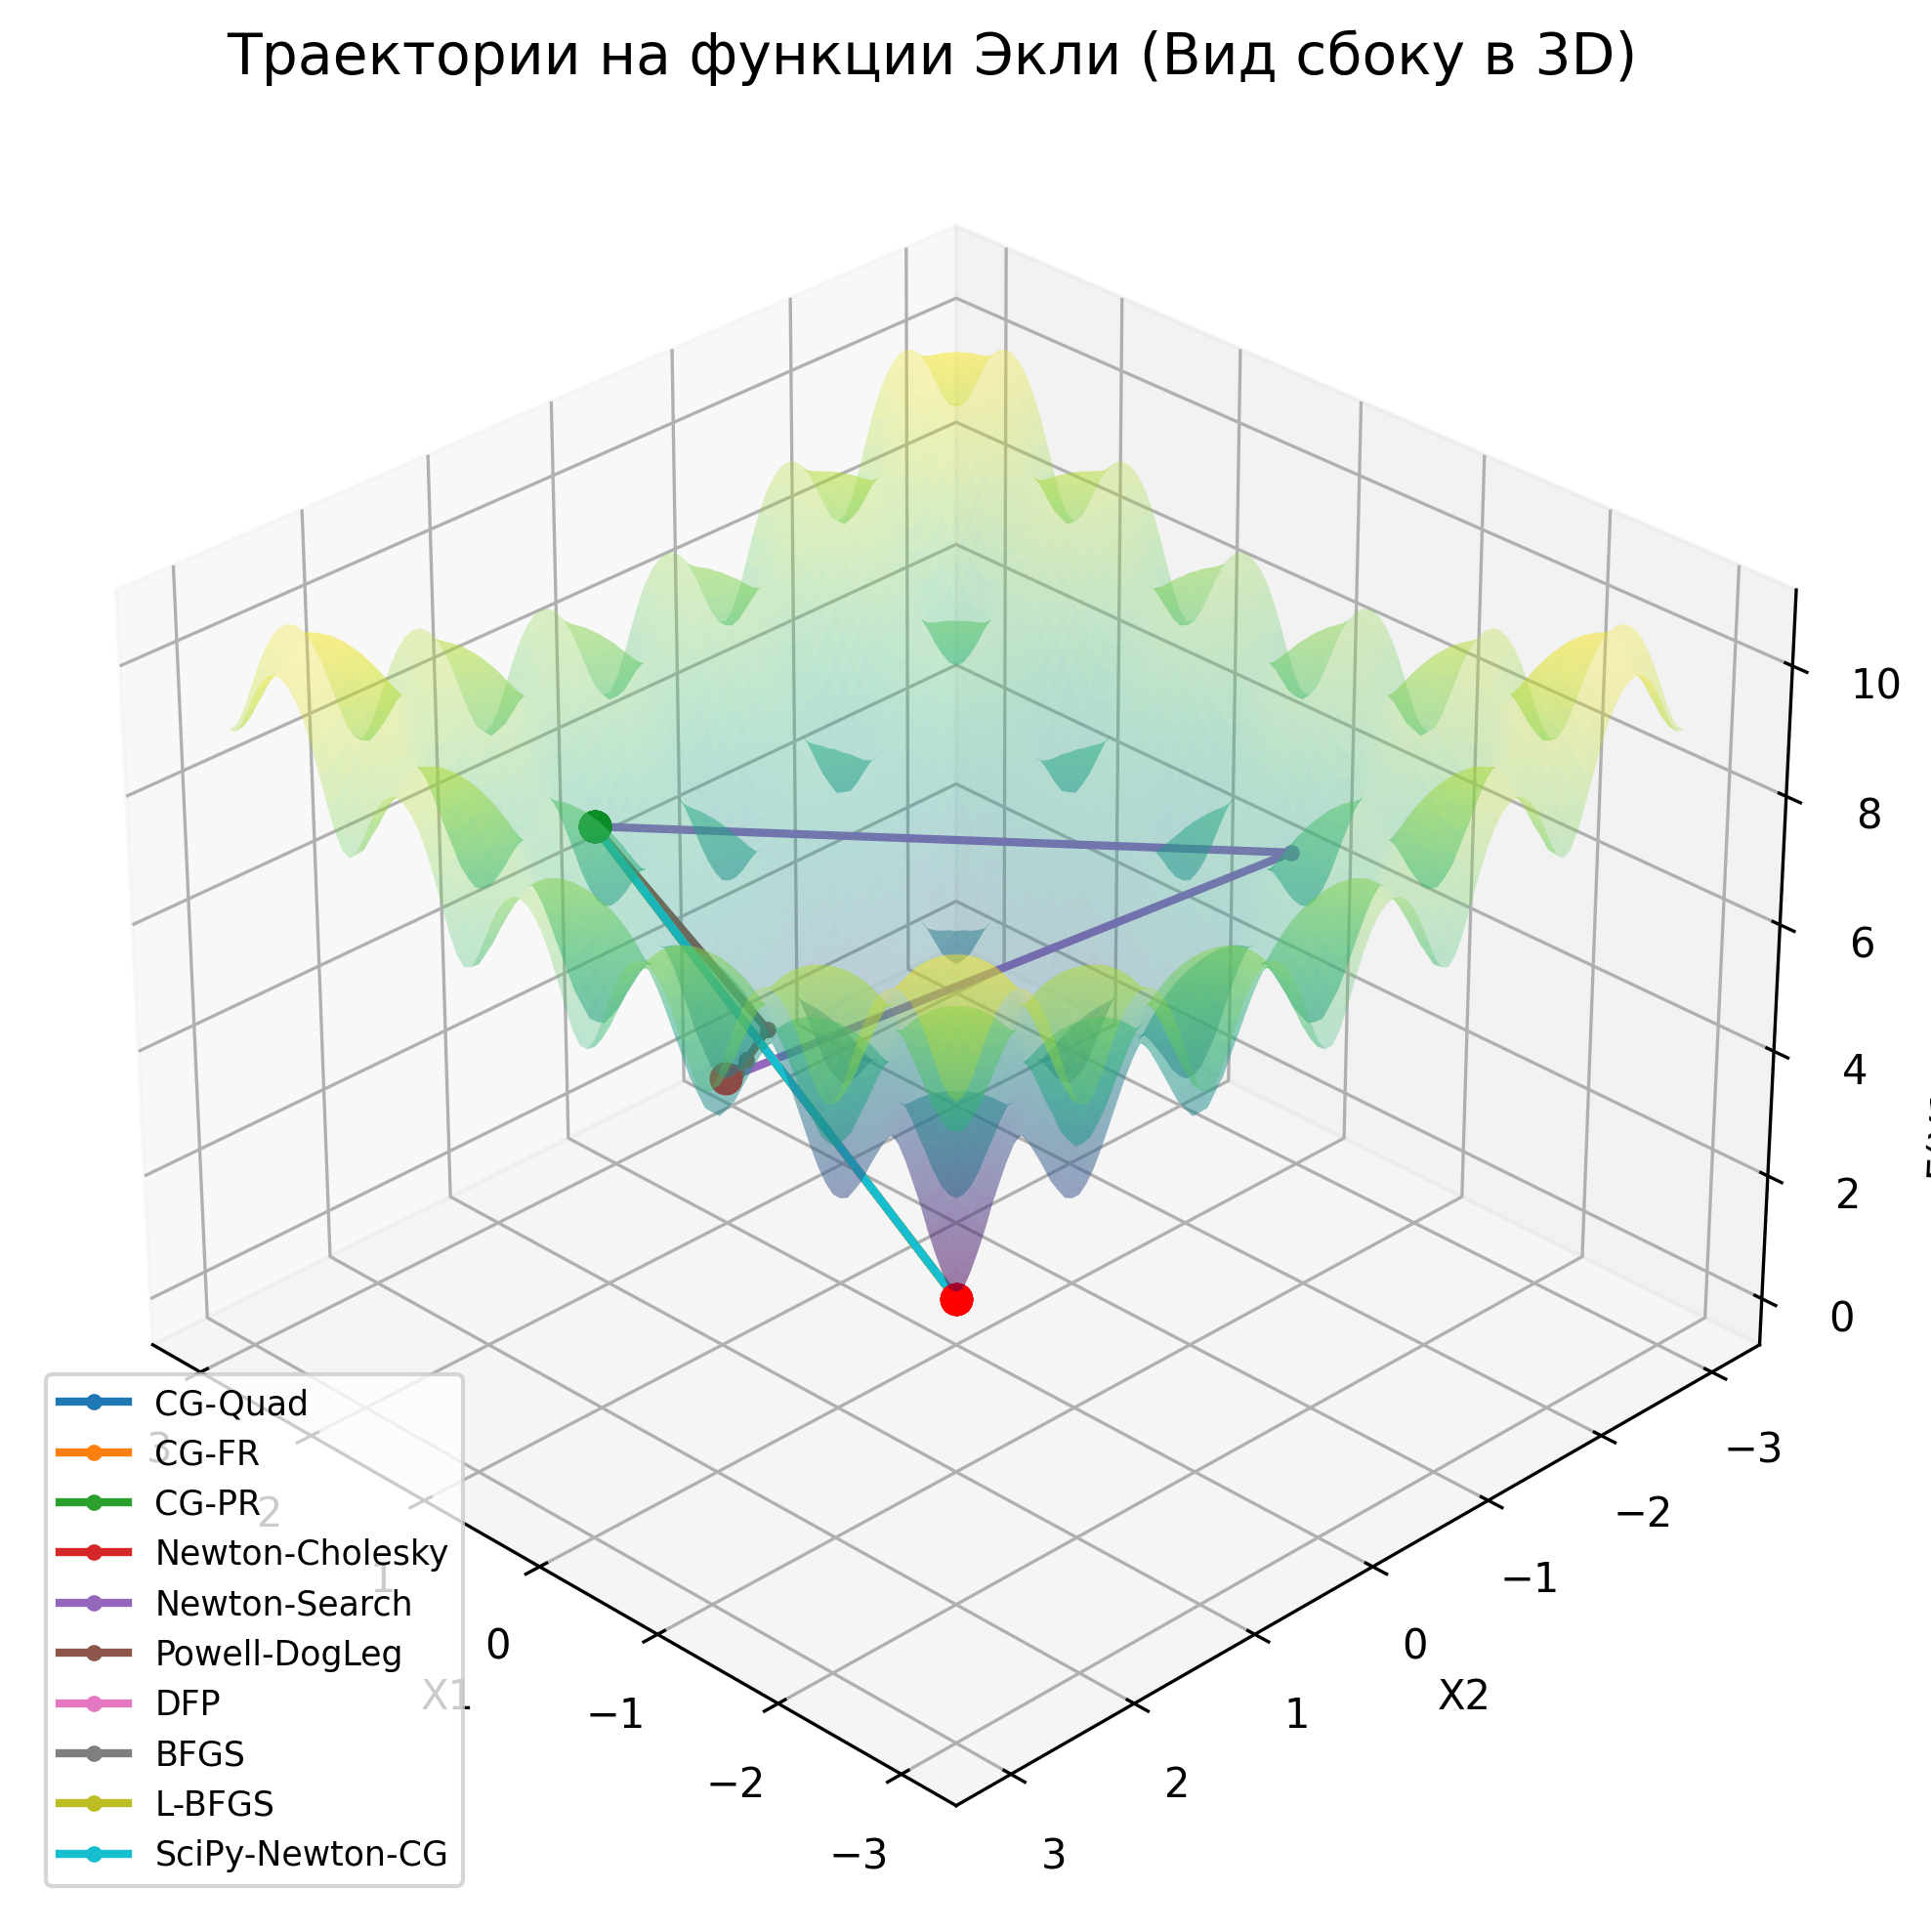
\includegraphics[width=\textwidth]{results/plots/ackley_trajectory_3d_side.png}
        \caption{Экли сбоку}
    \end{subfigure}
    \caption{Траектории методов на линиях уровня сложных функций. На Розенброке видно, как методы
    второго порядка проходят дно долины; на Химмельблау траектории расходятся к разным минимумам;
    на Экли часть методов застревает в локальном минимуме вблизи $(0.97, 0.97)$.}
    \label{fig:complex}
\end{figure}

% ─────────────────────────────────────────────────────────────
\subsection{\texorpdfstring{Задание 4: влияние размера памяти $m$ в L-BFGS}{Задание 4: влияние размера памяти m в L-BFGS}}
% ─────────────────────────────────────────────────────────────

Серия запусков L-BFGS на квадратичной задаче ($n=50$, $k=100$, $x_0 = (3,\dots,3)^\top$) при
$m \in \{1, 2, 5, 10, 20, 50\}$.

\input{results/tables/lbfgs_memory.tex}

\paragraph{Вывод.}
Увеличение памяти $m$ монотонно сокращает число итераций: с 81 при $m=1$ до 41 при $m=20$. Однако
эффект быстро насыщается — переход от $m=20$ к $m=50$ (полная память при $n=50$) уже не даёт
выигрыша. Это типичное поведение L-BFGS: нескольких последних пар $(s_i, y_i)$ достаточно, чтобы
восстановить основную кривизну, а хранить всю историю (что эквивалентно BFGS) невыгодно по памяти.
Практический компромисс $m = 5\text{--}10$ обеспечивает близкое к BFGS число итераций при затратах
памяти $O(mn) \ll O(n^2)$. Метки $\times$ снова отражают остановку по стагнации на уровне машинного
шума, а не сбой метода.

\begin{figure}[H]
    \centering
    \includegraphics[width=0.65\textwidth]{results/plots/fig_lbfgs_memory.png}
    \caption{Зависимость числа итераций L-BFGS от размера памяти $m$ ($n=50$, $k=100$). Кривая
    быстро выходит на плато: после $m \approx 10$ дополнительная память почти не ускоряет метод.}
    \label{fig:lbfgs_memory}
\end{figure}

% ═════════════════════════════════════════════════════════════
\section{Сравнительный анализ методов}
% ═════════════════════════════════════════════════════════════

\paragraph{Число итераций против суммарной стоимости.}
Малое число итераций не означает малой вычислительной стоимости. Методы Ньютона сходятся за
1 итерацию на квадратике, но каждая итерация требует вычисления и разложения гессиана ($O(n^3)$).
Линейный CG не трогает $H_f^{-1}$ вовсе и обходится одним вычислением $A$, но делает до $n$
итераций. Квазиньютоновские методы не вычисляют гессиан совсем (столбцы $H_f$ равны нулю), а
платят несколькими вычислениями $f$ и $\grad f$ на шаг из-за Вольфе-поиска. Поэтому при сравнении
методов нужно смотреть на все пять учётных столбцов одновременно, а не только на число итераций.

\paragraph{Влияние числа обусловленности.}
\begin{itemize}
    \item \textbf{Сопряжённые направления.} Линейный CG конечен ($\leq n$ шагов) при любом $k$,
          но фактическая скорость управляется $\sqrt{\kappa}$. Нелинейные CG чувствительны к $k$:
          их число итераций растёт примерно как $\sqrt{\kappa}$ (FR: $28 \to 106$ при росте $k$ от
          10 до $10^3$).
    \item \textbf{Методы Ньютона.} Аффинно инвариантны: на квадратике дают 1 шаг \emph{независимо}
          от $k$. Обусловленность влияет лишь на устойчивость разложения, но не на число итераций.
    \item \textbf{Квазиньютоновские методы.} Занимают промежуточное положение: накапливают
          информацию о кривизне за несколько итераций, поэтому зависят от $k$ слабее, чем
          первопорядковые CG, но сильнее, чем Ньютон.
\end{itemize}

\paragraph{Требование положительной определённости гессиана.}
\begin{itemize}
    \item \textbf{Требуют $H_f \succ 0$:} немодифицированный Ньютон по Холецкому (иначе разложение
          невозможно — остановка со статусом) и линейный CG (иначе $p^\top A p \leq 0$).
    \item \textbf{Устойчивы к нарушению:} Ньютон с выбором направления (регуляризация
          $H_f + \tau I$) и Dog Leg (доверительная область ограничивает шаг при невыпуклой модели).
    \item \textbf{Поддерживают $\succ 0$ по построению:} DFP, BFGS, L-BFGS сохраняют
          $H_k \succ 0$ при условии кривизны $\inner{s_k}{y_k} > 0$, обеспечиваемом Вольфе, и потому
          всегда дают направление спуска.
\end{itemize}
Эксперимент с Экли в точке с неопределённым гессианом прямо иллюстрирует это разделение.

% ═════════════════════════════════════════════════════════════
\section{Общие выводы}
% ═════════════════════════════════════════════════════════════

\begin{enumerate}
    \item \textbf{Квадратичные/выпуклые задачи.} Если гессиан доступен и положительно определён,
          метод Ньютона вне конкуренции (1 итерация, аффинная инвариантность). При больших $n$,
          когда $O(n^3)$ дорого, выгоднее линейный CG (нет работы с $H_f^{-1}$) или BFGS.

    \item \textbf{Число обусловленности — ключевой параметр для первого порядка.} Нелинейные CG
          замедляются как $\sqrt{\kappa}$, тогда как методы Ньютона к $\kappa$ нечувствительны.
          На плохо обусловленных задачах предпочтительны методы второго порядка и квазиньютоновские.

    \item \textbf{Большая размерность.} L-BFGS даёт почти ту же скорость, что BFGS, при затратах
          памяти $O(mn)$; памяти $m = 5\text{--}10$ практически достаточно — кривая числа итераций
          выходит на плато.

    \item \textbf{Сложные нелинейные функции.} Устойчивее всего ведут себя методы с защитой от
          невыпуклости: Ньютон с регуляризацией, Dog Leg и квазиньютоновские методы.
          Немодифицированный Ньютон по Холецкому останавливается на неположительно определённом
          гессиане, а линейный CG применим лишь к квадратичным задачам.

    \item \textbf{Многоэкстремальность и причины остановки.} На функции Экли разные методы
          приходят к разным исходам — глобальный минимум, локальный минимум, остановка по
          неопределённости гессиана или по стагнации. Единый формат результата с явной причиной
          остановки позволяет корректно различать эти случаи, что и требовалось в работе.
\end{enumerate}

\end{document}
